\documentclass[english]{panikzettel}

\newcommand{\classP}{\textsf{P}}
\newcommand{\classNP}{\textsf{NP}}
\usetikzlibrary{patterns}

\usepackage{graphicx}
\newcommand{\subpoint}[0]{\rotatebox[origin=c]{180}{$\Lsh$}~}

\usepackage{environ} % alignat* won't work with newenvironment
\NewEnviron{linearprogram}{%
  \begin{alignat*}{3}
    \BODY
  \end{alignat*}
  \vspace{-1.8\baselineskip}
}
\newcommand{\lpAnnotation}[1]{\ifx&#1&{}\else\text{\footnotesize{}(#1)}\fi}
\newcommand{\lpVars}[3]{\text{\textcolor{gray}{Variables: }} & #1 \quad && #2 \quad & \lpAnnotation{#3}\\[0.8em]}
\newcommand{\lpMoreVars}[3]{\\[-2.2em] & #1 \quad && #2 \quad & \lpAnnotation{#3}\\[0.8em]}
\newcommand{\lpMin}[1]{\text{min} \quad & #1 \\}
\newcommand{\lpMax}[1]{\text{max} \quad & #1 \\}
\newcommand{\lpWhere}[3]{\text{\textcolor{gray}{where}} \quad & #1 \quad && #2 \quad & \lpAnnotation{#3} \\}
\newcommand{\lpConstraint}[3]{ & #1 \quad && #2 \quad & \lpAnnotation{#3} \\}

\title{Logistics Systems Planning 1 Panikzettel}
\author{Philipp Schröer, Luca Oeljeklaus}

\begin{document}
\maketitle

\tableofcontents

\section{Introduction}

This Panikzettel is about the lecture Logistics Systems Planning 1 by Prof.\ Schneider held in the winter semester 2019/20 and is based on the corresponding slides.

This Panikzettel is Open Source. We appreciate comments and suggestions at \\ \url{https://git.rwth-aachen.de/philipp.schroer/panikzettel}.
\bigskip

In this Panikzettel, we introduce new notation for better readability: $\overline{n} := \set{1,\ldots, n}$ for some $n$.

\section{Logistic Systems}

Logistic activities include:
\begin{itemize}
    \item \emph{Supply logistics}: managing raw materials, parts, etc.,
    \item \emph{Internal logistics}: stocking, transportation between facilities, packaging, etc.,
    \item \emph{Distribution logistics}: supplying of sales points, anything between production and sale.
\end{itemize}

Planning of a logistics system can be split into three decision levels: \emph{strategic}, \emph{tactical}, and \emph{operational}.

\begin{halfboxl}
    \small{}
    \textbf{Storage}
    \begin{itemize}
        \item Strategic:
            \begin{itemize}
                \item Warehouse planning,
                \item Selection of warehouse equipment,
                \item Choice of warehouse layout.
            \end{itemize}
        \item Tactical:
            \begin{itemize}
                \item Product allocation at storage points,
                \item Choice of inventory policies.
            \end{itemize}
        \item Operational:
            \begin{itemize}
                \item Warehouse picking,
                \item Consolidation in loading area.
            \end{itemize}
    \end{itemize}
\end{halfboxl}%
\begin{halfboxr}
    \vspace{-\baselineskip}
    \small{}
    \textbf{Distribution}
    \begin{itemize}
        \item Strategic:
            \begin{itemize}
                \item Choice of transport mode,
                \item Fleet size and composition.
            \end{itemize}
        \item Tactical:
            \begin{itemize}
                \item Freight assigment,
                %\item Network design,
                \item Vehicle assignment,
                \item Crew rostering.
            \end{itemize}
        \item Operational:
            \begin{itemize}
                \item Vehicle routing,
                \item Positioning of vehicles and containers,
                \item Consolidation of orders.
            \end{itemize}
    \end{itemize}
\end{halfboxr}

\section{Graph Theory}

\subsection{Graphs}

\begin{halfboxl}
    \vspace{-\baselineskip}
    \begin{defi}{Undirected Graph}
        An \emph{undirected graph} $G = (V,~ E)$ consists of
        \begin{itemize}[leftmargin=*]
            \item a \emph{vertex set} $V$, and
            \item \emph{edges} $E \subseteq \Set{\set{v,w} \in V^2 | v \neq w}$.
        \end{itemize}
        \medskip

        \small{}
        The \emph{star} (incident edges) of a vertex $v$ is
        \begin{tightcenter}
          $\delta(v) = \Set{ \set{v,w} \in E }$.
        \end{tightcenter}

        The \emph{degree} of a vertex $v$ is $d(v) = \abs{\delta(v)}$.

        The set of \emph{neighbours} of a vertex $v$ is
        \begin{tightcenter}
            $\Delta(v) = N(v) = \Set{w \in V| \Set{v,w} \in E}$.
        \end{tightcenter}
    \end{defi}

    A \emph{mixed graph} $G = (V, A, E)$ consists of both directed and undirected edges.
    A \emph{multigraph} is an undirected graph with potentially multiple edges between two nodes.
\end{halfboxl}%
\begin{halfboxr}
    \vspace{-\baselineskip}
    \begin{defi}{Directed Graph}
        A \emph{directed graph} (\emph{digraph}) $G = (V,~ A)$:
        \begin{itemize}[leftmargin=*]
            \item a \emph{vertex set} $V$, and
            \item \emph{arcs} $A \subseteq \Set{ (v,w) | v,w \in V,~ v \neq w }$.
        \end{itemize}
        \medskip

        \small{}
        The \emph{backward star} (incoming arcs) of $v$ is
        \begin{tightcenter}
            $\delta^-(v) = \Set{(w,v) \in A|w \in V}$.
        \end{tightcenter}
        \subpoint \emph{forward star} $\delta^+(v)$ with outgoing arcs.

        The \emph{in-degree} of $v$ is $d^-(v) = \abs{\delta^-(v)}$.\\
        \subpoint Similar with \emph{out-degree} $d^+(v)$.

        The set of \emph{predecessors} of $v$ is given by
        \begin{tightcenter}
            $\Delta^-(v) = N^-(v) = \Set{w \in V| (w,v) \in E}$.
        \end{tightcenter}
        \subpoint Similar with \emph{successors} $\Delta^+(v)$.
    \end{defi}
\end{halfboxr}
\vspace{-0.5\baselineskip}

The \emph{underlying graph} of a graph is obtained by removing the direction of its edges. The number of edges stays the same.
A \emph{Hamiltonian path} in an undirected graph visits all nodes exactly once.

An \textbf{undirected graph} is \emph{Eulerian} if for every vertex $v$, $d(v)$ is even.

A \textbf{directed graph} is Eulerian if for every vertex $v$ it holds that $d^-(v) = d^+(v)$.

A \textbf{mixed graph} is Eulerian if the sum of all degrees is even and for every vertex set $S \subset V$ it holds that $|d^-(S) - d^+(S)| \le d^u(S)$.
This basically states that for any vertex set, either we have the same number of in- and outgoing edges or we have enough undirected edges to compensate the lack of in- or outgoing edges.

A \emph{strong (weak) component} is a maximum set of nodes which are mutually reachable via directed (undirected) paths.

\begin{halfboxl}
    \vspace{-15pt}

    \subsection{Minimum Spanning Tree}

    A \emph{minimum spanning tree} is a subset of edges in an \textbf{undirected graph} with edge weights, so that the subset is a tree (all nodes are connected by exactly one path) and with minimum edge weight.

    The idea of \emph{Prim's Algorithm} is to select an arbitrary start node and to iteratively build a set of ``reached'' vertices which at the end should include all vertices.

    In every iteration, it looks at the star (set of incident edges) of the ``reached'' vertex set, that is, all edges that have one endpoint in the set and one outside and selects the one with the lowest weight.
    It then adds the newly reached vertex to the set.

    \emph{Kruskal's algorithm} on the other hand sorts all vertices by increasing weights.
    Then it always selects the next smallest edge that it can be added to the current tree without introducing a cycle.
    Should this not be the case, the edge is discarded.
    The algorithm terminates when $n-1$ edges have been selected.

    \subsection{Shortest Paths}

    There are different algorithms to find shortest paths in graphs: either between two nodes, between one node and all others, or between all pairs of nodes.

    \emph{Dijkstra's algorithm} computes the shortest path between one node and all other nodes in a graph.

    The algorithm keeps track of a distance $d(v)$ and a predecessor $pred(v)$ for each node $v$.
    Starting from $s$, we keep updating the distances and predecessors of neighbours of a node.
    If a node was updated, we mark it so its own neighbours will be visited again.
    We do this until no node is marked (no changes happened).
\end{halfboxl}%
\begin{halfboxr}
    \vspace{-\baselineskip}
    \begin{algo}{Prim}
        \textbf{Input:} Graph $G = (V, E)$ with weights.

        \textbf{Output:} MST $T \subseteq E$.
        \tcblower
        \begin{enumerate}
            \item Let $T \leftarrow \set{ \set{v,w} }$ where $\set{v,w}$ is the cheapest edge.
            \item Until $\bigcup T = V$ (all vertices reached):
                \begin{itemize}
                    \item Find cheapest edge $\set{v,w}$ that connects a new node {\small{}($\abs{\set{v,w} \cap \bigcup T} = 1$)}.
                    \item Set $T \leftarrow T \cup \Set{ \set{v,w} }$.
                \end{itemize}
            \item Return $T$.
        \end{enumerate}
    \end{algo}

    \begin{algo}{Kruskal}
        \textbf{Input:} Graph $G = (V, E)$ with weights.

        \textbf{Output:} MST $T \subseteq E$.
        \tcblower
        \begin{enumerate}
            \item Let $T \leftarrow \emptyset$.
            \item Until $\abs{T} = \abs{V} - 1$:
                \begin{itemize}
                    \item Take next cheapest edge $\set{u,v} \notin T$.
                    \item If \texttt{is\_acyclic($T \cup \set{u,v}$)}, then
                        \begin{itemize}
                            \item $T \leftarrow T \cup \Set{ \set{u,v} }$.
                        \end{itemize}
                    \end{itemize}
            \item Return $T$.
        \end{enumerate}
    \end{algo}

    \begin{algo}{Dijkstra}
        \textbf{Input:} Weighted graph $G = (V, E)$ with weights $w(i,j) \in \nat$, and a source $s \in V$.

        \textbf{Output:} A predecessor function $pred$ and a distance function $d$.
        \tcblower
        \begin{enumerate}
            \item $d(s) \leftarrow 0$ and $d(j) = \infty ~~\Forall j \in V \setminus \{s\}$.
            \item Set $pred(s) \leftarrow 0$.
            \item Set $L \leftarrow \set{s}$.
            \item While $L \neq \emptyset$:
                \begin{enumerate}
                    \item Select $i \leftarrow \argmin_{k \in L} d(k)$.
                    \item Set $L \leftarrow L \setminus \set{i}$.
                    \item {\small{}Each $j \in N(i)$ with $d(j) > d(i) + w(i,j)$:}
                    \begin{itemize}
                        \item Set $d(j) \leftarrow d(i) + w(i,j)$,
                        \item Set $pred(j) \leftarrow i$,
                        \item Add $L \leftarrow L \cup \set{j}$.
                    \end{itemize}
                \end{enumerate}
            \item Return $pred$ and $d$.
        \end{enumerate}
    \end{algo}
\end{halfboxr}


\section{Location Planning}

Location planning is done on either \emph{continuous} or \emph{discrete} location spaces.
Then there is the distinction into \emph{single-commodity} and \emph{multi-commodity location problems}.
Finally, we can also have \emph{single-echelon location problems} with flow only in one direction (as opposed to \emph{two-echelon location problems}).

\subsection{Qualitative Methods}

\begin{halfboxl}
    \emph{Qualitative methods} can be used if the number of solutions is discrete and small.

    The \emph{weighted scoring method} weighs a set of facilities $V$ by $m$ \emph{location factors}.
	Each factor $k$ has a weight $w_k \in (0,1)$, and each facility $i$ has a score $s_{ik}$.
	The weights are assumed to sum up to $1$.
\end{halfboxl}%
\begin{halfboxr}
	\vspace{-\baselineskip}
	\begin{algo}{Weighted scoring method}
		\textbf{Input:} A set $V$ of facilities, and weights $w_1,\ldots,w_m$, and scores $s_{ik}$.

		\textbf{Output:} Preferred site $i^\ast$.
		\tcblower
		\begin{enumerate}
			\item For every site $i \in V$, calculate
				\begin{tightcenter}
					$r_i = \sum_{k=1}^m w_k s_{ik}$.
				\end{tightcenter}
			\item $i^\ast = \argmax_{i \in V} r_i$.
		\end{enumerate}
	\end{algo}
\end{halfboxr}
\vspace{-\baselineskip}

\subsection{Continuous SESC}

\begin{halfboxl}
    The \emph{(continuous) single-echelon single-commodity (SESC)} location problem is to find the optimal location of a single facility in a two-dimensional Cartesian plane (L2-metric) with a single commodity that is to be supplied to a set of successor nodes.

    We basically want to find a ``central'' point that has least overall distances where nodes can have different weights.
    Note that the transport cost $c$ is completely irrelevant for the problem.

    For the continuous SESC problem, there is an ugly analytical \textbf{and recursive} expression:
	\begin{align*}
		x^\ast &= \frac{\sum_{i \in V} \left( \frac{d_i x_i}{\sqrt{(x_i - x^\ast)^2 + (y_i - y^\ast)^2}} \right)}{\sum_{i \in V} \left( \frac{d_i}{\sqrt{(x_i - x^\ast)^2 + (y_i - y^\ast)^2}} \right)} \\
		y^\ast &= \text{(analogous)}
	\end{align*}

    We can heuristically approach this result by doing a fixpoint iteration called \emph{Weiszfeld heuristic}: To calculate $x^\ast$ (respectively $y^\ast$), start with the ``average point'', and then plug in the formulas above recursively until the error threshold $\varepsilon$ is reached.
    For $\varepsilon = 0$, this heuristic is actually exact.
\end{halfboxl}%
\begin{halfboxr}
	\vspace{-\baselineskip}
	\begin{defi}{Continuous SESC}
		In the \emph{single-echelon single-commodity location problem}, we have a \emph{transport cost} $c$ and for each node $i \in V$:
		\begin{itemize}
			\item coordinates $(x_i,y_i)$,
			\item a demand $d_i$.
		\end{itemize}
        We want to find the optimal location of the new facility $(x,y) = \argmin_{(x,y) \in \mathbb{R}^2} f(x,y)$ where
        {\small{}
		\[
			f(x,y) = \sum_{i \in V} c \cdot d_i \cdot \left( \sqrt{(x_i - x)^2 + (y_i - y)^2} \right).
		\]}
    \end{defi}

    \begin{algo}{Weiszfeld heuristic}
		(SESC input and output)
		\tcblower
		\begin{enumerate}
			\item Start with $x^0 = \frac{\sum_{i \in V} d_i x_i}{\sum_{i \in V} d_i}$ and analogously for $y^0$.
			\item Iteratively compute $x^{(h+1)}$ ($y^{(h+1)}$) by
				\[
					x^{(h+1)} = \frac{\sum_{i \in V} \left( \frac{d_i x_i}{\sqrt{(x_i - x^h)^2 + (y_i - y^h)^2}} \right)}{\sum_{i \in V} \left( \frac{d_i}{\sqrt{(x_i - x^h)^2 + (y_i - y^h)^2}} \right)}
                \]
				until {\small{}$f(x^{(h+1)}, y^{(h+1)}) - f(x^{(h)}, y^{(h)}) \leq \varepsilon$}.
		\end{enumerate}
	\end{algo}
\end{halfboxr}

\subsection{Discrete SESC}

\begin{halfboxl}
    In the discrete \emph{single-echelon single-commodity location problem (SESC)}, we work on a complete bipartite graph.
    We now also add a maximum facility output $q_i$ for each facilities $i \in V_1$, because why not.
    We also add a production cost $F_i$ for each facility $i$.

    It is also possible to add a time horizon $1,\ldots,T$ and make facility outputs time-dependent ($q_{it}$); similar for demands.
\end{halfboxl}%
\begin{halfboxr}
    \vspace{-\baselineskip}
    \begin{defi}{Discrete SESC}
        In the \emph{single-echelon single-commodity location problem}, we are given
        \begin{itemize}
            \item a complete directed bipartite graph $G = (V_1 \cup V_2, A)$, with facilities $V_1$ and clients $V_2$ and arcs $A = V_1 \times V_2$,
            \item a maximum output $q_i$ for $i \in V_1$,
            \item a demand $d_j$ for $i \in V_2$,
            \item a transport cost $C_{ij}(s)$ for $s \in \nat$,
            \item a production cost $F_i(s)$ for $s \in \nat$.
        \end{itemize}
    \end{defi}
\end{halfboxr}
\vspace{-\baselineskip}
\begin{linearprogram}
  \lpVars{s_{ij} \ge 0}{\Forall i \in V_1, \Forall j \in V_2}{delivery quantity from $i$ to $j$}
  \lpMoreVars{u_{i} \ge 0}{\Forall i \in V_1}{production at facility $i$}
  \lpMin{\sum_{i \in V_1} \sum_{j \in V_2} C_{ij}(s_{ij}) + \sum_{i \in V_1} F_i(u_i)}
  \lpWhere{\sum_{j \in V_2} s_{ij} = u_i}{\Forall i \in V_1}{every facility $i$ ships exactly all it produces}
  \lpConstraint{\sum_{i \in V_1} s_{ij} = d_j}{\Forall j \in V_2}{every client $j$ receives its demand}
  \lpConstraint{\sum_{j \in V_2} s_{ij} \le q_i}{\Forall i \in V_1}{facility output limit}
\end{linearprogram}

An instance in this category is the \emph{capacitated plant location problem}.
The \emph{simple plant location problem} does not have maximum outputs for facilities.

\subsubsection[p-Median Model]{$p$-Median Model}

The \emph{$p$-median model} is a discrete SESC model with a few simplifications.
We want to find exactly $p$ facility locations and have a fixed cost $c_{ij} \geq 0$ for each facility $i \in V_1$ that supplies $j \in V_2$.
\begin{linearprogram}
  \lpVars{x_{ij} \in \Set{0,1}}{\Forall i \in V_1, \Forall j \in V_2}{$x_{ij} = 1$ iff $i$ supplies $j$}
  \lpMoreVars{y_{i} \in \Set{0,1}}{\Forall i \in V_1}{$y_i = 1$ iff facility $i$ is opened}
  \lpMin{\sum_{i \in V_1} \sum_{j \in V_2} c_{ij} x_{ij}}
  \lpWhere{\sum_{i \in V_1} x_{ij} = 1}{\Forall j \in V_2}{every client $j$ is connected to one facility}
  \lpConstraint{\sum_{j \in V_2} x_{ij} \leq \abs{V_2} \cdot y_i}{\Forall i \in V_1}{facility $i$ can only serve if opened}
  \lpConstraint{\sum_{i \in V_1} y_i = p}{}{exactly $p$ facilities opened}
\end{linearprogram}

\subsubsection{Demand Allocation Problem}

In the \emph{demand allocation problem}, we want to find out \textbf{average quantities} to be supplied for a fixed set of facilities $\overline{V_1}$.
\begin{linearprogram}
    \lpVars{0 \leq x_{ij} \leq 1}{\Forall i \in \overline{V_1}, \Forall j \in V_2}{$x_{ij}$ is the average supply from $i$ to $j$}
    \lpMin{\sum_{i \in \overline{V_1}} \sum_{j \in V_2} c_{ij} \cdot x_{ij} + \sum_{i \in \overline{V_1}} f_i}
    \lpWhere{\sum_{i \in \overline{V_1}} x_{ij} = 1}{\Forall j \in V_2}{averages sum to $1$}
    \lpConstraint{\sum_{j \in V_2} d_j \cdot x_{ij} \leq q_i}{\Forall i \in \overline{V_1}}{facility output limit}
\end{linearprogram}

\subsection{Location-Covering Problem}

In the \emph{location-covering problem}, we want to cover a set of users $V_2$ by a subset of facilities $V_1$ in a graph $G = (V_1 \cup V_2,~ A)$ with edges $A$.
We minimise fixed costs of selected facilities $f_i \Forall i \in V_1$, while having each user being served by at least one facility to which it is connected. This is expressed by boolean constants $a_{ij} ~\Forall i \in V_1, j \in V_2$ which is 1 if the edge from $i$ to $j$ exists.
\begin{linearprogram}
  \lpVars{y_i \in \Set{0,~1}}{\Forall i \in V_1}{$y_i = 1$ iff facility $i$ is opened}
  \lpMin{\sum_{i \in V_1} f_i \cdot y_i}
  \lpWhere{\sum_{i \in V_1} a_{ij} \cdot y_i \ge 1}{\Forall j \in V_2}{at least one serving facility per client}
\end{linearprogram}

\subsubsection{LCP Heuristic}

\begin{algo}{Location-Covering Problem Heuristic}
    \textbf{Input:} An LCP instance.

    \textbf{Output:} A set of facilities to be opened.
    \tcblower
    {\small{}%
    Define \textbf{open($i$)}:
    \begin{itemize}
        \item Open $i$: Set $y_i = 1$.
        \item Mark $i$'s neighbours as covered: Delete all constraints containing $a_{ij} \cdot y_i$ where $a_{ij} = 1$.
    \end{itemize}}

    \begin{enumerate}
        \item Construct the LCP LP above.
        \item While there are still constraints left:
        \begin{enumerate}
            \item For facility $i$ that is free (where $f_i = 0$):
                \begin{itemize}
                    \item \textbf{open($i$)}.
                \end{itemize}
            \item For facility $i$ that is not connected ($a_{ij} = 0~ \Forall j \in V_2$) and not free:
                \begin{itemize}
                    \item \textbf{close($i$)}: Set $y_i = 0$.
                \end{itemize}
            \item Find facility $i$ that is cheapest per covered neighbour ($\argmin_i f_i/n_i$): \\
                {\small{}($n_i$ is the number of constraints $y_i$ appears in, i.e. the number of covered neighbours.)}
                \begin{itemize}
                    \item \textbf{open($i$)}.
                \end{itemize}
        \end{enumerate}
        \item Return $\Set{ i \in V_1 | y_i =1 }$.
    \end{enumerate}
\end{algo}

\subsubsection[p-Center Problem]{$p$-Center Problem}

In a \emph{$p$-center problem}, we want to locate exactly $p$ facilities so that the maximum travel time from a user to the closest facility is minimised.
The $p$ facilities are either on vertices or arcs/edges on a (potentially mixed) graph $G = (V, E, A)$.
This problem is \textsf{NP}-hard for $p \ge 2$. If $G$ is directed, then there is an optimal solution with the facilities located solely on vertices.

\begin{minipage}[t]{0.475\textwidth}
    The \emph{$1$-center problem} is solved by \emph{Hakimi's algorithm}.
    Here, we have travel times $t_{ij}$ from node $i$ to $j$.
    Then we have a distance function $\tau_h : P \to \mathbb{R}$ that maps a set of points $P = \set{p_{hk}, \ldots | \set{h,k} \in E}$ to a distance.
    These points lie somewhere on the edges (but may also lie directly on one vertex).
    \medskip

    \begin{center}
        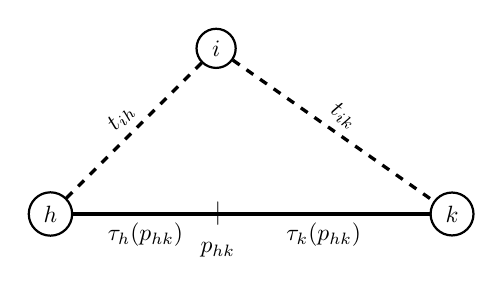
\begin{tikzpicture}[scale=0.85, every node/.style={transform shape}]
            \node[fill=white,draw=black,circle,thick] (h) [] {$h$};
            \node[fill=white,draw=black,circle,thick] (k) [right of=h,node distance = 6cm] {$k$};
            \node[fill=white,draw=black,circle,thick] (i) [above right of=h,node distance = 3.5cm] {$i$};
            \node[fill=none,draw=none] (p) [right of=h, node distance=2.5cm,label={below:$p_{hk}$}] {$|$};

            \draw [very thick]  (h) edge []     node [sloped,below] {$\tau_h(p_{hk})$} (p.center)
                                (p.center) edge []     node [sloped,below] {$\tau_k(p_{hk})$} (k)
                                (h) edge [dashed]     node [sloped,above] {$t_{ih}$} (i)
                                (i) edge [dashed]     node [sloped,above] {$t_{ik}$} (k);
        \end{tikzpicture}
    \end{center}
    \medskip

    The travel time from one point $p_{hk}$ on the edge ${h,k}$ to a vertex $i$ is given by $T_i(p_{hk})$.
    The algorithm first computes minimal travel times from every point to every vertex.
    Then, for every edge ${h,k}$, the best $p_{hk}$ is selected.
    Finally, we choose the best of those over all edges.
\end{minipage}\hspace*{0.025\textwidth}%
\begin{minipage}[t]{0.5\textwidth}
    \vspace{-\baselineskip}
    \definecolor{prussianblue}{rgb}{0.0, 0.19, 0.33}
    \begin{algo}{Hakimi}
            \textbf{Input:}
                \begin{itemize}[leftmargin=\leftmargini]
                    \item A graph $G = (V,E)$,
                    \item distances $\tau_h : P \to \mathbb{R}$
                    \item for points {\small{}$P = \set{p_{hk}, \ldots | \set{h,k} \in E}$}.
                \end{itemize}

            \raggedright{}
            \textbf{Output:} A point $p_{hk}$.
        \tcblower
        \begin{enumerate}[leftmargin=*]
            \item \textbf{Minimal travel times} for every vertex $i \in V$ to any point on the edge $\Set{h,k}$:
                \vspace{-0.5\baselineskip}
                {\small{}
                \begin{align*}
                    T_i : P &\to \mathbb{R} \\
                    T_i(p_{hk}) &= \min \Set{ t_{ih} + \tau_h(p_{hk}),~ t_{ik} + \tau_k(p_{hk}) }
                \end{align*}}
            \item \textbf{Local center} for every edge, the point that minimises {\color{prussianblue}the maximum distance to all vertices}:
                \vspace{-0.5\baselineskip}
                $$p^*_{hk} = \argmin_{p_{hk} \in P} {\color{prussianblue}\max_{i \in V} T_i(p_{hk})}.$$
            \item \textbf{Find 1-center}, the best local center:
                \vspace{-0.5\baselineskip}
                $$p^* = \argmin_{p_{hk} \in P} {\color{prussianblue}\max_{i \in V} T_i(p^*_{{hk}})}.$$
        \end{enumerate}
    \end{algo}
\end{minipage}

\section{Transportation Planning}

\subsection{Modes of Transport}

\paragraph{Rail Transport}
Rail transport is inexpensive, but slow and unreliable. This is due to: It having a lower priority than passenger rail, direct connections being rare, and requiring a large quantity of goods in order to be profitable. It is mostly used to transport raw materials.

\vspace{-\baselineskip}
\paragraph{Road Transport}
Road transport is mostly used to transfer (semi-)finished products using trucks and can be separated into two categories, \emph{truckload (TL)} and \emph{less-than-truckload (LTL)}.
TL is used to transfer directly from one location to another using the full capacity of the vehicle.
LTL is used when single shipments are significantly smaller than vehicle capacity.
Shipments are then transfered between vehicles covering different legs of the trip.

\vspace{-\baselineskip}
\paragraph{Air Transport}
Air transport is fast, but slowed by airport handling, and only competitive for long-haul transport.
Planes have very low capacity.
Thus they are mostly used for high-value goods over long distance.

\vspace{-\baselineskip}
\paragraph{Water Transport}
Water transport is mostly used to send bulk raw materials, represents $99\%$ of the weight and $50\%$ of the value of international trade.
Also it's pretty cheap.

\vspace{-\baselineskip}
\paragraph{Pipeline Transport}
Pipeline transport only usable for specific goods, very slow, can provide a constant flow of goods, and is very reliable.

\subsection{Vehicle Routing Problems}

\begin{halfboxl}
    In \emph{Vehicle Routing Problems (VRPs)}, we want to route $m$ vehicles on a graph, starting and ending at a depot $o \in V$.
    Usually, we minimise costs of edges/arcs and number of vehicles used.
    \begin{itemize}[leftmargin=*]
        \item \hyperref[sec:nrp]{\ref*{sec:nrp}: \emph{Node Routing Problem (NRP)}} \\ {\small{}if $R = \emptyset$ (only target vertices)}
            \begin{itemize}
                \item \emph{Traveling Salesperson Problem (TSP)} \\ {\small{}if $m = 1$ (one vehicle)}
            \end{itemize}
        \item \hyperref[sec:arp]{\ref*{sec:arp}: \emph{Arc Routing Problem (ARP)}} \\ {\small{}if $U = \emptyset$ (only target arcs/edges)}
            \begin{itemize}
                \item \emph{Rural Postman Problem (RPP)} \\ {\small{}if $m = 1$ (one vehicle)}
                \begin{itemize}
                    \item \emph{Chinese Postman Problem (CPP)} \\ {\small{}if $G$ is complete}
                \end{itemize}
            \end{itemize}
    \end{itemize}
\end{halfboxl}%
\begin{halfboxr}
    \vspace{-\baselineskip}
    \begin{defi}{Vehicle Routing Problem}
            A instance of a VRP is defined on a graph $G = (V,A,E)$ with:
            \begin{itemize}[nosep]
                \item $V$: a vertex set,
                \item $A$: a directed edge set,
                \item $E$: an undirected edge set,
                \smallskip
                \item $o \in V$: the origin,
                \item $U \subseteq V$: the target vertices,
                \item $R \subseteq A \cup E$: the target arcs/edges,
                \item $m$: number of vehicles,
                \smallskip
                \item (some costs to minimise).
        \end{itemize}
    \end{defi}
\end{halfboxr}
\vspace{-\baselineskip}

Note: Often, the term \emph{Vehicle Routing Problem} is used to refer to NRPs.
ARPs are explicitly named.

\subsection{Node Routing Problems (NRPs)}
\label{sec:nrp}

\subsubsection{Traveling Salesperson Problem (TSP)}

In the \emph{traveling salesperson problem}, we want to find a route for one vehicle that visits all required vertices and the depot.
The input graph $G$ is not necessarily complete, so we consider the auxiliary complete graph $G' = (V', A')$ where $V' = U \cup \Set{0}$ and $(i,j) \in A'$ with costs $c_{ij}$, the cost of the least-cost path between $i$ and $j$.

$G'$ satisfies the triangle inequality: $c_{ij} \leq c_{ik} + c_{kj} \quad \Forall (i,j) \in A',~ k \in V',~ k \neq j, j$.

\vspace{-\baselineskip}
\begin{linearprogram}
    \lpVars{x_{ij} \in \Set{0,1}}{\Forall (i,j) \in A'}{$x_{ij} = 1$ iff $(i,j)$ is part of the solution}
    \lpMin{\sum_{(i,j) \in A'} c_{ij} \cdot x_{ij}}
    \lpWhere{\sum_{i \in V' \setminus \Set{j}} x_{ij} = 1}{\Forall j \in V'}{every vertex $j$ has an incoming arc}
    \lpConstraint{\sum_{j \in V' \setminus \Set{i}} x_{ij} = 1}{\Forall i \in V'}{every vertex $i$ has an outgoing arc}
    \lpConstraint{\sum_{i,j \in S} x_{ij} \leq \abs{S} - 1}{\Forall S \subsetneq V',~ \abs{S} \geq 2}{subtour elimination constraints}
\end{linearprogram}

\emph{Asymmetric TSP (ATSP)} as presented above is $\classNP$-hard.
We can obtain a lower bound by solving the \emph{assignment problem}, a relaxation of ATSP.
The idea is to remove the subtour elimination constraints and the integrality of $x_{ij}$ (so that only $x_{ij} \geq 0$).
Additionally, set $c_{ii} = \infty \quad \Forall i \in V'$ so that $x_{ii}^\ast = 0$.
Then the optimal solution of the LP (solvable in polynomial time!) represents a collection of subtours in $G'$ over all vertices.
This gives us a lower bound for the optimal cost of ATSP.

\subsubsection{Capacitated VRP (CVRP)}

We refer to our \href{https://panikzettel.philworld.de/or1.pdf}{Operations Research 1 Panikzettel} which has a section on VRP.

\subsubsection{VRP with Time Windows (VRPTW)}

We refer to our \href{https://panikzettel.philworld.de/or1.pdf}{Operations Research 1 Panikzettel} which has a section on VRP.

\subsection{VRP/NRP Heuristics}

\subsubsection{Patching Heuristic}

The \emph{patching heuristic} is useful for the ATSP, and the solutions it yields for the STSP are pretty bad.
This is due to the fact that solving the STSP LP without SECs yields a lot of tours of length 2.

We solve the ATSP LP without the SECs.
All edges in the optimal solution are on at exactly one tour.
Then the two subtours with the largest number of nodes are merged so that the overall cost is least increased.
Repeat until we have only one tour left.

\subsubsection{Nearest Neighbour Heuristic}

Select a start node.
Always select nearest neighbour to continue the tour.
If vehicle capacity is reached, end tour and start over with next vehicle.

\subsubsection{Insertion Heuristics}

\emph{Insertion heuristics} add heuristically chosen nodes to the current subtour.
One may start with a tour of three nodes, for example the largest triangle.
\begin{itemize}
    \item \emph{Nearest insertion}: Select vertex closest to any vertex already in the tour.
    \item \emph{Cheapest insertion}: Greedily select vertex that is cheapest to insert.
    \item \emph{Farthest insertion}: Select the farthest vertex from any vertex in the tour.
    \item \emph{Random insertion}: Add a randomly chosen vertex.
\end{itemize}
Nearest and cheapest insertion are $2$-approximations, while farthest and random insertion are only $6.5$-approximations.
On empirical examples however, farthest and random insertion perform better than the two others.

\pagebreak
\subsubsection{CVRP Construction Heuristics}

There are two types of \emph{construction heuristics} given $m$ vehicles:
\begin{itemize}
    \item Cluster first, route second: Partition vertices into $m$ clusters and then solve the STSP on each induced complete subgraph (exactly or heuristically).
    \item Route first, cluster second: Compute a single route and then split into $m$ feasible subroutes.
\end{itemize}

\subsubsection{Savings Heuristic}

The \emph{savings heuristic} is for symmetric VRP only.
Start by connecting every vertex by an individual tour to the origin.
Then compute for every pair of tours the \emph{savings}: what we would save by fusing that pair of tours compared to having two separate tours.
After sorting all pairs of tours by decreasing savings, repeatedly fuse the pair which provides the most savings, until no more positive savings can be found.

\begin{algo}{Savings Heuristic}
\textbf{Input:} A graph $G = (V,E,c)$ with $c:E\to\mathbb{Q}^+$. \\
\textbf{Output:} A set of tours $C$.
\tcblower
\begin{enumerate}[nosep]
    \item Compute the set $C$ of $n$ tours $C_i \coloneqq (0,i,0)$ for all $i \in V$.
    \item For every pair of vertices $v$ and $w$ with $v \neq w$:
        \begin{itemize}
            \item compute \textbf{potential savings} $s_{vw} = c_{0v} + c_{w0} - c_{vw}$.
        \end{itemize}
    \item Let $L$ be the sorted list of savings that are \textbf{non-negative}.
    \item While $L$ is non-empty:
    \begin{enumerate}
        \item Select the first feasible element $(v,w)$ of $L$. $(v,w)$ is feasible if
            \begin{itemize}
                \item $v$ is the \textbf{last vertex of its tour},
                \item and $w$ \textbf{the first of its own} (or vice versa) and,
                \item if applicable, if the current vehicle \textbf{meets the capacity requirements}.
            \end{itemize}
        \item Remove all unfeasible edges from $L$.
        \item Remove $(v,0)$ and $(0,w)$ and fuse the tours $C_v$ and $C_w$ by adding the edge $(v,w)$.
    \end{enumerate}
    \item Return $C$.
\end{enumerate}
\end{algo}

\subsubsection[k-opt Local Search Heuristic]{$k$-opt Local Search Heuristic}

Given a heuristic solution to a node routing problem, the \emph{$k$-opt heuristic} can be used to further improve the solution.
The idea is to explore all similar solutions and choose a better one.
Here, we choose the best solution among all those where $k$ edges are substituted by $k$ other edges.
Repeatedly do this until the solution cannot be improved in this way.
Then we have a local optimum.
The heuristic has exponential runtime in $k$ and thus usually $k = 2$ or $k = 3$.

\subsection{Arc Routing Problems}
\label{sec:arp}

\begin{halfboxl}
    In \emph{arc routing problems (ARP)}, one has to traverse a (sub-)set of arcs in a graph at least once.
    ARPs are classified by two aspects.

    \vspace{-\baselineskip}
    \paragraph{Link type and weight} \textbf{(U)}~undirected, \textbf{(D)}~directed, \textbf{(M)}~mixed (i.e.\ both directed and undirected), and \textbf{(W)}~windy, where edges always have a reverse edge, but the cost is not necessarily symmetric ($c_{ij} \neq c_{ji}$).

    \vspace{-\baselineskip}
    \paragraph{Connection of links} The \emph{Chinese postman problem (CPP)} is defined on connected graphs.
    Otherwise we have a \emph{pural postman problem (RPP)}.
\end{halfboxl}%
\begin{halfboxr}
    \small{}
    \begin{center}
        \begin{tabular}{r|c|c|}
             & Chinese Postman & Rural Postman \\ \hline
            U & UCPP (\classP) & URPP (\classNP) \\ \hline
            D & DCPP (\classP) & DRPP (\classNP) \\ \hline
            M & MCPP (\classNP) & MRPP (\classNP) \\ \hline
            W & WCPP (\classNP) & WRPP (\classNP) \\ \hline
        \end{tabular}

        (Only directed and undirected Chinese Postman Problems are solvable in polynomial time.)
    \end{center}
\end{halfboxr}

\section{Warehouse Planning}
\subsection{Warehouse Layouts}
\begin{halfboxl}
    Here, we go through three different types of warehouse layouts, which are illustrated on the right.
    The first one is the \emph{flow-through layout}, with one end of the warehouse having entry points, the other having exit points, and the storage lying inbetween. This layout is useful if most load units require the same operations.

    The \emph{U-layout}, illustrated in the middle, describes a situation in which entry and exit points are on the same side of the warehouse. It is useful for low material flows and when needing flexibility with regards to the assignment of shipping/receiving space.

    The \emph{hybrid layout} has entry and exit points on different, though non-opposed sides of the building.
\end{halfboxl}%
\begin{halfboxr}
    \vspace{-1.8\baselineskip}
    \begin{center}
        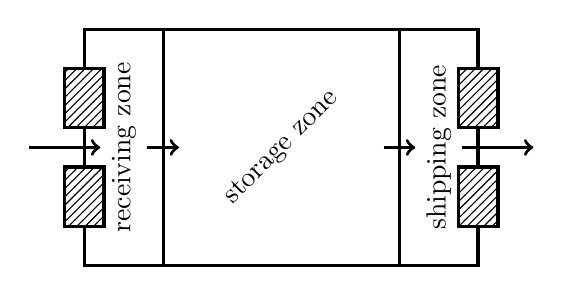
\begin{tikzpicture}[draw=black,fill=white,very thick]
            \draw[fill=white] (0,0) rectangle (5,3) node[pos=.5] {\rotatebox{45}{storage zone}};
            \draw[fill=white] (0,0) rectangle (1,3) node[pos=.5] {\rotatebox{90}{receiving zone}};
            \draw[fill=white] (4,0) rectangle (5,3) node[pos=.5] {\rotatebox{90}{shipping zone}};

            \draw[fill=white] (-0.25,0.5) rectangle (0.25,1.25);
            \draw[fill=white] (-0.25,1.75) rectangle (0.25,2.5);
            \draw[fill=white] (4.75,0.5) rectangle (5.25,1.25);
            \draw[fill=white] (4.75,1.75) rectangle (5.25,2.5);
            \draw[pattern=north east lines,draw=none] (-0.25,0.5) rectangle (0.25,1.25);
            \draw[pattern=north east lines,draw=none] (-0.25,1.75) rectangle (0.25,2.5);
            \draw[pattern=north east lines,draw=none] (4.75,0.5) rectangle (5.25,1.25);
            \draw[pattern=north east lines,draw=none] (4.75,1.75) rectangle (5.25,2.5);

            \draw[->] (-0.7,1.5) -- (0.2,1.5);
            \draw[->] (0.8,1.5) -- (1.2,1.5);
            \draw[->] (3.8,1.5) -- (4.2,1.5);
            \draw[->] (4.8,1.5) -- (5.7,1.5);
        \end{tikzpicture}
    \end{center}
    \begin{center}
        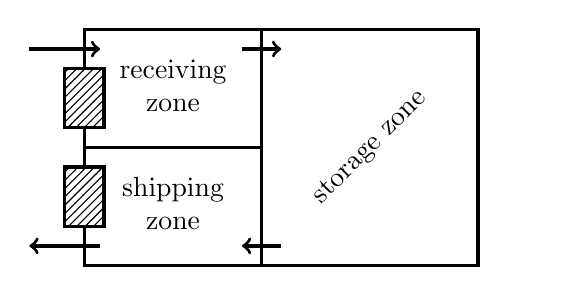
\begin{tikzpicture}[draw=black,fill=white,very thick]
            \draw[fill=white] (2.25,0) rectangle (5,3) node[pos=.5] {\rotatebox{45}{storage zone}};
            \draw[fill=white] (0,0) rectangle (2.25,1.5) node[pos=.5] {\rotatebox{0}{\begin{tabular}{c} shipping \\ zone
            \end{tabular}}};
            \draw[fill=white] (0,1.5) rectangle (2.25,3) node[pos=.5] {\rotatebox{0}{\begin{tabular}{c} receiving \\ zone
            \end{tabular}}};
            \draw[fill=white] (-0.25,0.5) rectangle (0.25,1.25);
            \draw[fill=white] (-0.25,1.75) rectangle (0.25,2.5);
            \draw[pattern=north east lines,draw=none] (-0.25,0.5) rectangle (0.25,1.25);
            \draw[pattern=north east lines,draw=none] (-0.25,1.75) rectangle (0.25,2.5);

            \draw[->] (-0.7,2.75) -- (0.2,2.75);
            \draw[->] (2,2.75) -- (2.5,2.75);
            \draw[->] (2.5,0.25) -- (2,0.25);
            \draw[->] (0.2,0.25) -- (-0.7,0.25);
            \draw[->,draw=none] (4.8,1.5) -- (5.7,1.5); % for aligning purposes only
        \end{tikzpicture}
    \end{center}
    \begin{center}
        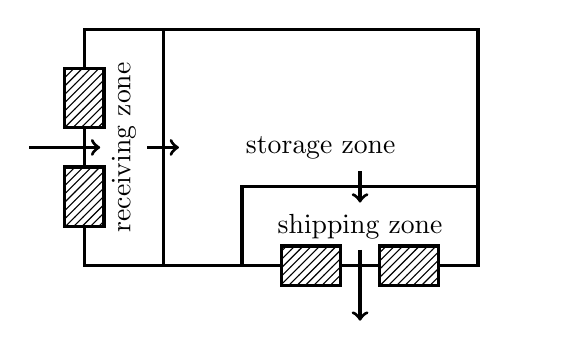
\begin{tikzpicture}[draw=black,fill=white,very thick]
            \draw[fill=white] (1,0) rectangle (5,3) node[pos=.5] {\rotatebox{0}{storage zone}};
            \draw[fill=white] (0,0) rectangle (1,3) node[pos=.5] {\rotatebox{90}{receiving zone}};
            \draw[fill=white] (2,0) rectangle (5,1) node[pos=.5] {\rotatebox{0}{shipping zone}};

            \draw[fill=white] (-0.25,0.5) rectangle (0.25,1.25);
            \draw[fill=white] (-0.25,1.75) rectangle (0.25,2.5);
            \draw[fill=white] (2.5,-0.25) rectangle (3.25,0.25);
            \draw[fill=white] (3.75,-0.25) rectangle (4.5,0.25);
            \draw[pattern=north east lines,draw=none] (-0.25,0.5) rectangle (0.25,1.25);
            \draw[pattern=north east lines,draw=none] (-0.25,1.75) rectangle (0.25,2.5);
            \draw[pattern=north east lines,draw=none] (2.5,-0.25) rectangle (3.25,0.25);
            \draw[pattern=north east lines,draw=none] (3.75,-0.25) rectangle (4.5,0.25);

            \draw[->] (-0.7,1.5) -- (0.2,1.5);
            \draw[->] (0.8,1.5) -- (1.2,1.5);
            \draw[->] (3.5,1.2) -- (3.5,0.8);
            \draw[->] (3.5,0.2) -- (3.5,-0.7);
            \draw[->,draw=none] (4.8,1.5) -- (5.7,1.5); % for aligning purposes only
        \end{tikzpicture}
    \end{center}
\end{halfboxr}

\begin{halfboxl}
    \vspace{-\baselineskip}
    \subsection{Picker Routing}
    The following descriptions of heuristics for efficient package picking will seem rather vague and informal. The author wants to apologise for this, however the material provided during the course of the lecture did not allow for a more precise write-up.
    \subsubsection{S-Shaped routing}
    \begin{enumerate}[nosep,leftmargin=*]
        \item From the entrance, move to the upmost row that contains packages.
        \item move down that row in an S-shape, entering only aisles that contain packages, traversing them completely.
        \item after having picked up the last package of the row, immediately rejoin the lower aisle.
        \item There, traverse the row in the same manner, choose direction freely.
        \item Continue until last row, then return to entrance.
    \end{enumerate}
    \subsubsection{Largest Gap Heuristic}
    \begin{enumerate}[nosep,leftmargin=*]
        \item For every aisle, compute the largest gap, that is, the largest distance between two packages or a package and an entrance such that no other package lies between. This gap shall not be crossed except if we reach the end of a row.
        \item Move to the upmost row that contains packages. Walk along the aisles and pick up all packages that can be reached without crossing the largest gap. Return when reaching the largest gap.
        \item After reaching the last aisle that contains a package, cross it completely and go in reverse, picking up packages that haven't been picked up.
    \end{enumerate}
    \subsubsection{Aisle-by-Aisle Heuristic}
    \begin{enumerate}[nosep,leftmargin=*]
        \item Starting from the leftmost aisle containing a package, traverse every aisle from left to right.
        \item Select crossaisle for traversal to minimise travel distance.
    \end{enumerate}
\end{halfboxl}%
\begin{halfboxr}
    \vspace{-\baselineskip}
    \begin{center}
        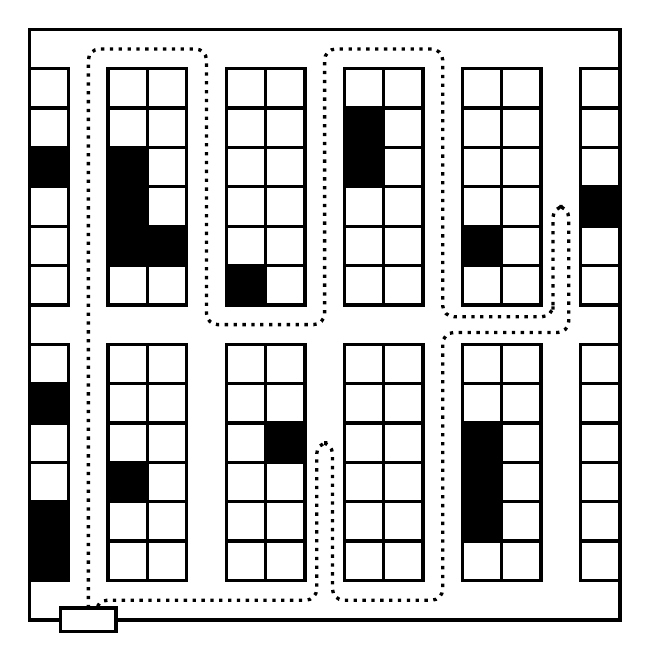
\begin{tikzpicture}[draw=black,fill=white,very thick]
            \draw [fill=white] (0,0) rectangle (7.5,7.5);
            \foreach \y in {0.5,1,1.5,2,2.5,3,4,4.5,5,5.5,6,6.5}
                \foreach \x in {0,1,1.5,2.5,3,4,4.5,5.5,6,7}
                    {\draw [fill=white] (\x,\y) rectangle (\x+.5,\y+.5);}

            % X % 0     1    1.5    2.5   3     4    4.5   5.5    6    7
            % Y % 0.5   1    1.5    2     2.5   3    4     4.5    5    5.5    6    6.5

            \draw [fill=black] (0,0.5) rectangle (0.5,1.5);
            \draw [fill=black] (0,2.5) rectangle (0.5,3);
            \draw [fill=black] (0,5.5) rectangle (0.5,6);

            \draw [fill=black] (1,1.5) rectangle (1.5,2);
            \draw [fill=black] (1,4.5) rectangle (1.5,6);

            \draw [fill=black] (1.5,4.5) rectangle (2,5);
            \draw [fill=black] (2.5,4) rectangle (3,4.5);

            \draw [fill=black] (3,2) rectangle (3.5,2.5);
            \draw [fill=black] (4,5.5) rectangle (4.5,6.5);
            \draw [fill=black] (5.5,1) rectangle (6,2.5);
            \draw [fill=black] (5.5,4.5) rectangle (6,5);
            \draw [fill=black] (7,5) rectangle (7.5,5.5);

            \draw [dotted,rounded corners]  (0.75,0.15) -- (0.75,7.25) --
                                            (2.25,7.25) -- (2.25,3.75) --
                                            (3.75,3.75) -- (3.75,7.25) --
                                            (5.25,7.25) -- (5.25,3.85) --
                                            (6.65,3.85) -- (6.65,3.85) --
                                            (6.65,5.25) -- (6.85,5.25) --
                                            (6.85,3.65) -- (5.25,3.65) --
                                            (5.25,0.25) -- (3.85,0.25) --
                                            (3.85,2.25) -- (3.65,2.25) --
                                            (3.65,0.25) -- (0.85,0.25) --
                                            (0.85,0.15);
            \draw [fill=white] (0.4,-0.15) rectangle (1.1,0.15);
        \end{tikzpicture}
    \end{center}
    \begin{center}
        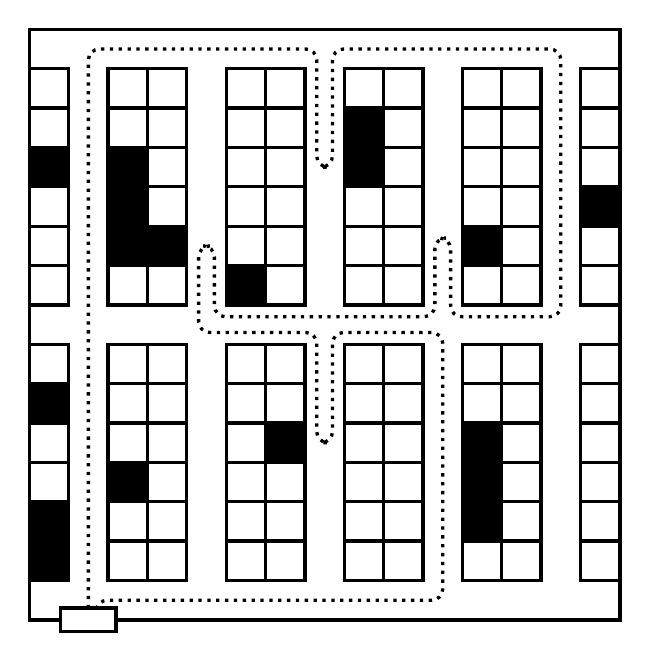
\begin{tikzpicture}[draw=black,fill=white,very thick]
            \draw [fill=white] (0,0) rectangle (7.5,7.5);
            \foreach \y in {0.5,1,1.5,2,2.5,3,4,4.5,5,5.5,6,6.5}
                \foreach \x in {0,1,1.5,2.5,3,4,4.5,5.5,6,7}
                    {\draw [fill=white] (\x,\y) rectangle (\x+.5,\y+.5);}

            % X % 0     1    1.5    2.5   3     4    4.5   5.5    6    7
            % Y % 0.5   1    1.5    2     2.5   3    4     4.5    5    5.5    6    6.5

            \draw [fill=black] (0,0.5) rectangle (0.5,1.5);
            \draw [fill=black] (0,2.5) rectangle (0.5,3);
            \draw [fill=black] (0,5.5) rectangle (0.5,6);

            \draw [fill=black] (1,1.5) rectangle (1.5,2);
            \draw [fill=black] (1,4.5) rectangle (1.5,6);

            \draw [fill=black] (1.5,4.5) rectangle (2,5);
            \draw [fill=black] (2.5,4) rectangle (3,4.5);

            \draw [fill=black] (3,2) rectangle (3.5,2.5);
            \draw [fill=black] (4,5.5) rectangle (4.5,6.5);
            \draw [fill=black] (5.5,1) rectangle (6,2.5);
            \draw [fill=black] (5.5,4.5) rectangle (6,5);
            \draw [fill=black] (7,5) rectangle (7.5,5.5);

            \draw [dotted,rounded corners]  (0.75,0.15) -- (0.75,7.25) --
                                            (3.65,7.25) -- (3.65,5.75) --
                                            (3.85,5.75) -- (3.85,7.25) --
                                            (6.75,7.25) -- (6.75,3.85) --
                                            (5.35,3.85) -- (5.35,4.85) --
                                            (5.15,4.85) -- (5.15,3.85) --
                                            (2.35,3.85) -- (2.35,4.75) --
                                            (2.15,4.75) -- (2.15,3.65) --
                                            (3.65,3.65) -- (3.65,2.25) --
                                            (3.85,2.25) -- (3.85,3.65) --
                                            (5.25,3.65) -- (5.25,0.25) --
                                            (0.85,0.25) -- (0.85,0.15);
            \draw [fill=white] (0.4,-0.15) rectangle (1.1,0.15);
        \end{tikzpicture}
    \end{center}
    \begin{center}
        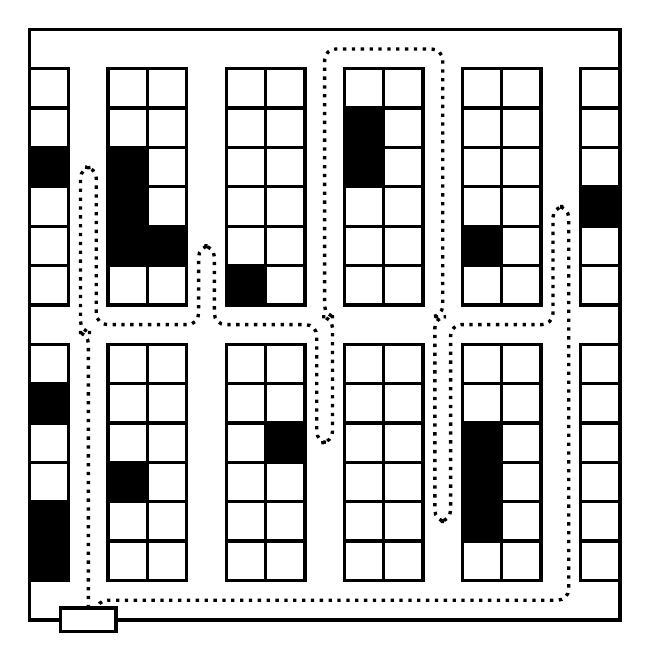
\begin{tikzpicture}[draw=black,fill=white,very thick]
            \draw [fill=white] (0,0) rectangle (7.5,7.5);
            \foreach \y in {0.5,1,1.5,2,2.5,3,4,4.5,5,5.5,6,6.5}
                \foreach \x in {0,1,1.5,2.5,3,4,4.5,5.5,6,7}
                    {\draw [fill=white] (\x,\y) rectangle (\x+.5,\y+.5);}

            % X % 0     1    1.5    2.5   3     4    4.5   5.5    6    7
            % Y % 0.5   1    1.5    2     2.5   3    4     4.5    5    5.5    6    6.5

            \draw [fill=black] (0,0.5) rectangle (0.5,1.5);
            \draw [fill=black] (0,2.5) rectangle (0.5,3);
            \draw [fill=black] (0,5.5) rectangle (0.5,6);

            \draw [fill=black] (1,1.5) rectangle (1.5,2);
            \draw [fill=black] (1,4.5) rectangle (1.5,6);

            \draw [fill=black] (1.5,4.5) rectangle (2,5);
            \draw [fill=black] (2.5,4) rectangle (3,4.5);

            \draw [fill=black] (3,2) rectangle (3.5,2.5);
            \draw [fill=black] (4,5.5) rectangle (4.5,6.5);
            \draw [fill=black] (5.5,1) rectangle (6,2.5);
            \draw [fill=black] (5.5,4.5) rectangle (6,5);
            \draw [fill=black] (7,5) rectangle (7.5,5.5);

            \draw [dotted,rounded corners]  (0.75,0.15) -- (0.75,3.65) --
                                            (0.65,3.65) -- (0.65,5.75) --
                                            (0.85,5.75) -- (0.85,3.75) --
                                            (2.15,3.75) -- (2.15,4.75) --
                                            (2.35,4.75) -- (2.35,3.75) --
                                            (3.65,3.75) -- (3.65,2.25) --
                                            (3.85,2.25) -- (3.85,3.85) --
                                            (3.75,3.85) -- (3.75,7.25) --
                                            (5.25,7.25) -- (5.25,3.85) --
                                            (5.15,3.85) -- (5.15,1.25) --
                                            (5.35,1.25) -- (5.35,3.75) --
                                            (6.65,3.75) -- (6.65,5.25) --
                                            (6.85,5.25) -- (6.85,0.25) --
                                            (0.85,0.25) -- (0.85,0.15)
                                            ;
            \draw [fill=white] (0.4,-0.15) rectangle (1.1,0.15);
        \end{tikzpicture}
        From top to bottom: S-shaped routing, Largest Gap Heuristic and Aisle-by-Aisle Heuristic.
    \end{center}
\end{halfboxr}

\end{document}
